\chapter{Research Results}
In this chapter, we will discuss the results of the research. We will discuss
the sampling algorithm for the Attraction Indian buffet process (AIBP) and
derive the p.m.f. of the distribution. Using a simulation study, we will also
compare the properties of the IBP, AIBP, and ddIBP.\\

\section{Notation for the AIBP}
Before discussing the sampling algorithm and the p.m.f. for the AIBP,  we will
discuss the notation that will be used. In this chapter, the term ``customer"
will be used to refer to a row (or observation) in a dataset; the term ``dish"
will likewise be used to refer to a column in a dataset. The terminology used
here is consistent with that used in the IBP and ddIBP.\\

\noindent
The order of customers in the dataset is not necessarily the order that the
observations will be assigned dishes in implementation. We will call $\bm
\sigma = (\sigma_1,..\sigma_n)$ the permutation of \textit{permutation} of the
data. The permutation gives the sequence in which the n customers are assigned
dishes, where the $t^{th}$ customer assigned is $\sigma_t$. Note that $\bm
\sigma = {1,...,n}$ when the customers are assigned in the order they appear
in the dataset.\\

\noindent
We will call $\lambda(i,j)$ the \textit{similarity} between customers $i$ and
$j$. The function $\lambda(\cdot)$ maps the distance between customers to a
measure of how ``close" together the customers are. If $d_{ij}$ represents the
distance between customers $i$ and $j$, then $\lambda(i,j)=f(d_{ij})$ should be
a non-increasing function such that $\lambda(0)>0$ and $\lambda(\infty)=0$. The
distance between customers should be non-negative. Examples of
$\lambda(i,j)=f(d_{ij})$ include: (i) reciprocal similarity $f(d) = 1/d$, and
(ii) exponential similarity $f(d) = exp(-d)$.\\

\noindent
We will let $x_i$ be the number of \textit{new} dishes that customer $i$ takes.
We will set $y_{-i} = \suml{j}{1}{i-1} x_j$, the number of existing dishes
before customer $i$ draws new dishes, for $i=\{2,...,N\}$. We will define
$y_{-i} = 0$. Note that $g_i(x_i) =
\ds\frac{(\alpha/i)^{x_i}\exp(-\alpha/i)}{x_i!}$, which is the probability mass
function for a Poisson distribution with parameter $\alpha/i$ and argument
$x_i$. We will let the number of (non-zero) columns in $\bm Z$ be $K$.
$m_{-i,k}$ = the number of customers that took dish $k$ before customer
customer $i$ samples dishes. We will let  $m_{-i} = \suml{k}{1}{K}m_{-i,k}$ be
the total number of dishes taken before customer $i$ samples any dishes.  We
will assign 
\[h_{i,k} = \hik,\]
the weight given to sampling dish $k$ for
customer $i$. The probability of customer $i$ drawing dish $k$ will be $p_{i,k}
= h_{i,k} \ds\frac{m_{-i}}{i}$. Note that when $\lambda$ is a constant,
$p_{i,k}$ reduces to $m_{-i,k}$ as in the IBP. We will define the harmonic
number to be $H_N = \suml{i}{1}{N} \ds\frac{1}{i}$.
%$h(i) = \prodl{k}{1}{y_{-i}} 
%(p_{i,k})^{z_{i,k}}(1-p_{i,k})^{1-z_{i,k}}$, for $i>1$,
%and $1$ for $i=1$.



\section{Sampling Algorithm for the AIBP}
We will now introduce the sampling algorithm for the AIBP for a given
permutation $\bm\sigma$. The sampling algorithm is similar to that of the IBP,
with minor changes to the sampling of previously sampled dishes. We will use 
$\bm Z$ to denote a realization from the AIBP with parameter $\alpha$, where 
$\alpha$ is a mass parameter that governs the number of dishes that will be drawn.
The larger $\alpha$ is, the larger the number of total dishes drawn ($K$) will be.\\

\noindent
To obtain a realization $\bm Z$ from an AIBP($\alpha$), the first customer
draws an $x_1 \sim$ Poisson($\alpha$) number of dishes. This is indicated by
setting $z_{1,1:x_1}$ to $1$. For each subsequent customer $i$, if there exists
any previously sampled dishes (i.e. if $y_{-i}>0$), customer $i$ samples dish
$k$ with probability $p_{i,k}$, for $k \in \{1,...,y_{-i}\}$. The customer then
samples an additional $x_i \sim$ Poisson($\alpha/i$) number of new dishes. 

%\begin{itemize}
%  \item The first customer draws an $x_1=$ Poisson($\alpha$) number of dishes. This
%        is indicated by setting $z_{1,1:x_1}$ to $1$.
%  \item For the next $i$ customers, for $i=1:N$, 
%     \begin{itemize}
%       \item if there exists previously sampled dishes, then customer $i$
%             samples dish k with probability $\left(h_{i,k}\right) 
%             \left(\ds\frac{m_{-i}}{i}\right)$, for $ k = 1:y_{-i}$.
%       \item customer $i$ draws another Poisson($\alpha/i$) number of new dishes.
%     \end{itemize}
%\end{itemize}

\section{Probability Mass Function}
Based on the sampling algorithm above, we can write down the p.m.f. for the
proposed distribution as a product of probabilities for each customer taking
each dish. Here we will define one more quantity:
$\prodl{k}{1}{y_{-i}} (p_{i,k})^{z_{i,k}}(1-p_{i,k})^{1-z_{i,k}}=1$ if $y_{-i}=0$.\\

\begin{align*}
  \text{P}(\bm Z|\bm\sigma)
  =&\prodl{i}{1}{N} \left\{g_i(x_i) \prodl{k}{1}{y_{-i}} 
    (p_{i,k})^{z_{i,k}}(1-p_{i,k})^{1-z_{i,k}}\right\}\\
  =&\prodl{i}{1}{N} \left\{ \ds\frac{(\alpha/i)^{x_i}\exp(-\alpha/i)}{x_i!} 
    \prodl{k}{1}{y_{-i}} 
    \ds\frac{(h_{i,k}m{-i})^{z_{i,k}}(i-h_{i,k}m_{-i,k})^{1-z_{i,k}}}{i} 
    \right\} \\
  =&\ds\frac{\alpha^{\suml{i}{1}{N}x_i} \exp(-\alpha H_N)} {\prodl{i}{1}{N}x_i!} 
    \left( \prodl{i}{1}{N}i^{-x_i} \right) \times
    \\
    &\left( \prodl{i}{1}{N}\prodl{k}{1}{y_{-i}} i^{-1}
    \ds\left(\hik m_{-i}\right)^{z_{i,k}}
       \left(i-\hik m_{-i}\right)^{1-z_{i,k}} \right)\\
   &\\
  =&\ds\frac{\alpha^K \exp(-\alpha H_N)} {\prodl{i}{1}{N}x_i!} \times
    \\
    &\left( \prodl{i}{2}{N} i^{-(x_i+y_{-i})}\prodl{k}{1}{y_{-i}} 
    \ds\frac{
    %\left(\sums{\sigma}{z_{-i,k}=1}{}\lambda(\sigma,\sigma_i)m_{-i}\right)^{z_{i,k}}
    %\left(i-\sums{\sigma}{z_{-i,k}=1}{}
    %\lambda(\sigma,\sigma_i)m_{-i}\right)^{1-z_{i,k}}
    \left(\suml{j}{1}{i-1}\lambda(\sigma_j,\sigma_i)z_{j,k}m_{-i}\right)^{z_{i,k}}
    \left(i-\suml{j}{1}{i-1}
    \lambda(\sigma_j,\sigma_i)z_{j,k}m_{-i}\right)^{1-z_{i,k}}
    }
    %{\suml{k}{1}{y_{-i}}\sums{\sigma}{z_{-i,k}=1}{}\lambda(\sigma,\sigma_i)}\right)
    {\suml{k}{1}{y_{-i}}\suml{j}{1}{i-1}\lambda(\sigma_j,\sigma_i)z_{j,k}}\right)
\end{align*}\\

\section{Properties of the AIBP}
In the literature review, it was shown how each of the mentioned distributions
that made use of pairwise distance information could be reduced to their original
distributions (CRP and IBP). The AIBP can likewise be reduced to the IBP when
the similarity function is constant (i.e. when f(d) = c, a constant).\\

\noindent
One of the properties we wished to preserve from the IBP was that the expected
number of dishes taken by each customer would be $\alpha$. The algorithm
prescribed above allocates dishes to customer based on their proximity to other
customers.  That is if two customers are close together, they are more likely
to share the same dishes. The number of new dishes sampled by each customer in
the AIBP is the same as that in the IBP (and is equal to $\alpha/i$), by
construction. So it remains to show that the expected number of
previously-sampled dishes $r_i$ sampled by customer $i$ in the AIBP is the
same as that in the IBP. In the IBP, the expected row sum for the first row is
$\alpha$, which is the same as in the AIBP. So the expected row sum is the same
for the first row. For subsequent rows, the expected value of $r_i$ in the IBP
is E$\left[\suml{k}{1}{y_{-i}} \frac{m_{-i,k}}{i}\right]$ =
E$\left[\frac{m_{-i}}{i}\right]$ = $\frac{\alpha(i-1)}{i}$. For the AIBP, the
expected value of $r_i$ is:
\[
  E\left[\suml{k}{1}{y_{-i}} h_{i,k} \frac{m_{-i}}{i}\right] = 
  E\left[\suml{k}{1}{y_{-i}}\hik \frac{m_{-i}}{i}\right] = 
  E\left[\frac{m_{-i}}{i}\right] = \frac{\alpha(i-1)}{i}
\]
Therefore, the expected row sums are the same for the AIBP and IBP. Note also
that since the mechanism for drawing new dishes is the same as that for the
IBP, the expected total number of dishes drawn, which is the total number of
non-zero columns $\bm Z$ is $\alpha+\alpha/1+...+\alpha/N = \alpha H_N$, as in
the IBP.  The implication is that the effective dimensions of the IBP are
preserved in the AIBP, but the assignment of dishes to customers is altered
by distance information.\\

\section{Simulation Study}
% Are observations close together really going to share the same dishes?
% Are distant observations going to disshare dishes?
% What are the next rows going to be, conditioned on the first few rows?
To better understand the behavior of the AIBP, a simulation study to compare
the IBP, AIBP, and ddIBP. We are particularly interested in three questions: 
(1) Do customers that are ``close" together tend to share similar dishes?
(2) Do customers that are ``far" away from one another tend to not share dishes?
(3) Given a particular arrangement for the first arbitrary number of customers,
how do subsequent customers choose dishes? 
\footnote{The simulation study can be accessed by installing and loading the
``shiny" package in R, then running the line: \\
> runGitHub(`shinyTest',`luiarthur')\\\\
The code for the simulation study can be viewed at: \\
https://github.com/luiarthur/shinyTest\\\\
A screen shot of the application used for the 
simulation study can be found in the appendix.}

\noindent
Through the simulation study, we were able to confirm that in simulation, the
AIBP reduces to the IBP when the similarity function is set to a constant (see
Figure 4.1).\\

\begin{figure}\begin{center}
  %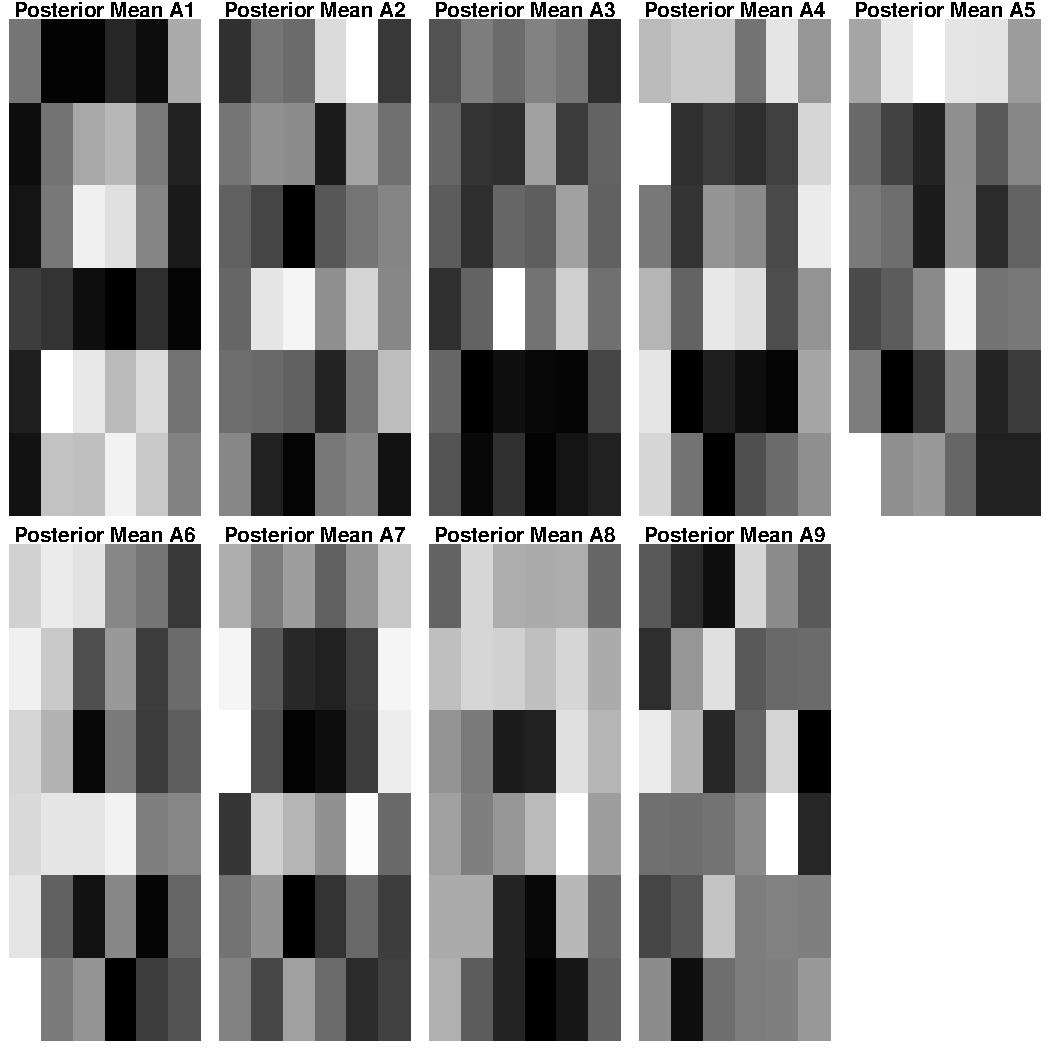
\includegraphics[height=1\textwidth]{images/postA66.pdf}
  \includegraphics{images/uni.pdf}
  \caption{The expected values of draws from the IBP were computed via simulation.
           Ten thousand realizations were drawn from the IBP with $\alpha=.5$.
           The ten thousand matrices were then summed across and divided by the
           number of realizations (10,000). Because draws from the IBP do not
           always have the same dimensions, each of the matrices were first padded
           with zeros to make matrix summation conformable. Expected values were
           computed in a similar way for the AIBP and ddIBP. In simulation, we
           have shown that the AIBP and ddIBP reduce to the IBP when the similarity
           function is set to a constant value. E[ncol] is the expected number of
           columns for a given distribution. Values in the cells of the matrices
           are the probabilities of those cells taking the value `1' as opposed
           to 0. The colors are an additional indication of the probabilities,
           red is used for cells with higher probability; white is used for cells
           with lower probability. The numbers to the left of the grids are the 
           expected row sums. The numbers at the bottom of the grids are the
           expected column sums.}
\end{center}\end{figure}
\noindent

Now we will examine the behavior of the AIBP using the distance matrix given in 
Table 4.1. This matrix is of particular interest because two pairs of customers
(1 \& 3, and 2 \& 5) are close together. All other customer pairings are distant.
One customer, customer 4, is far from every other customer. With these properties,
this matrix may provide some interesting insights into the behavior of the AIBP.
The similarity function used is the exponential function.\\

\begin{table}[ht]
\centering
\[
  \begin{pmatrix}{}
    0 & 9 & 1 & 9 & 9 \\ 
    9 & 0 & 9 & 9 & 1 \\ 
    1 & 9 & 0 & 9 & 9 \\ 
    9 & 9 & 9 & 0 & 9 \\ 
    9 & 1 & 9 & 9 & 0 \\ 
  \end{pmatrix}
\]
\caption{Distance Matrix used in this simulation study.}
\end{table}


\noindent
Figure 4.2 shows the expected value of the IBP, AIBP, and ddIBP simulated with
$\alpha=1.5$, and the distance matrix $D$ in Table 4.1. The three distributions
are clearly different. In the AIBP (middle), it is more probable for for the
$3^{rd}$ customer to take dish $1$, than it is in the IBP. This is reasonable
because the first customer tends to take the first dish frequently, and the
$3^{rd}$ customer is close to the first. In the ddIBP, customer $3$ is more likely
to take dish $1$ than any other customer. This is the main difference between the 
behavior of the AIBP and the ddIBP. The ddIBP takes into account the distance 
information of each customer to every other customer. In the AIBP, the distance 
information for only customers assigned prior to the current customer is made
use of. This may not necessarily be a desireable property, but it distinguishes 
the ddIBP from the AIBP.\\

\begin{figure}\begin{center}
  %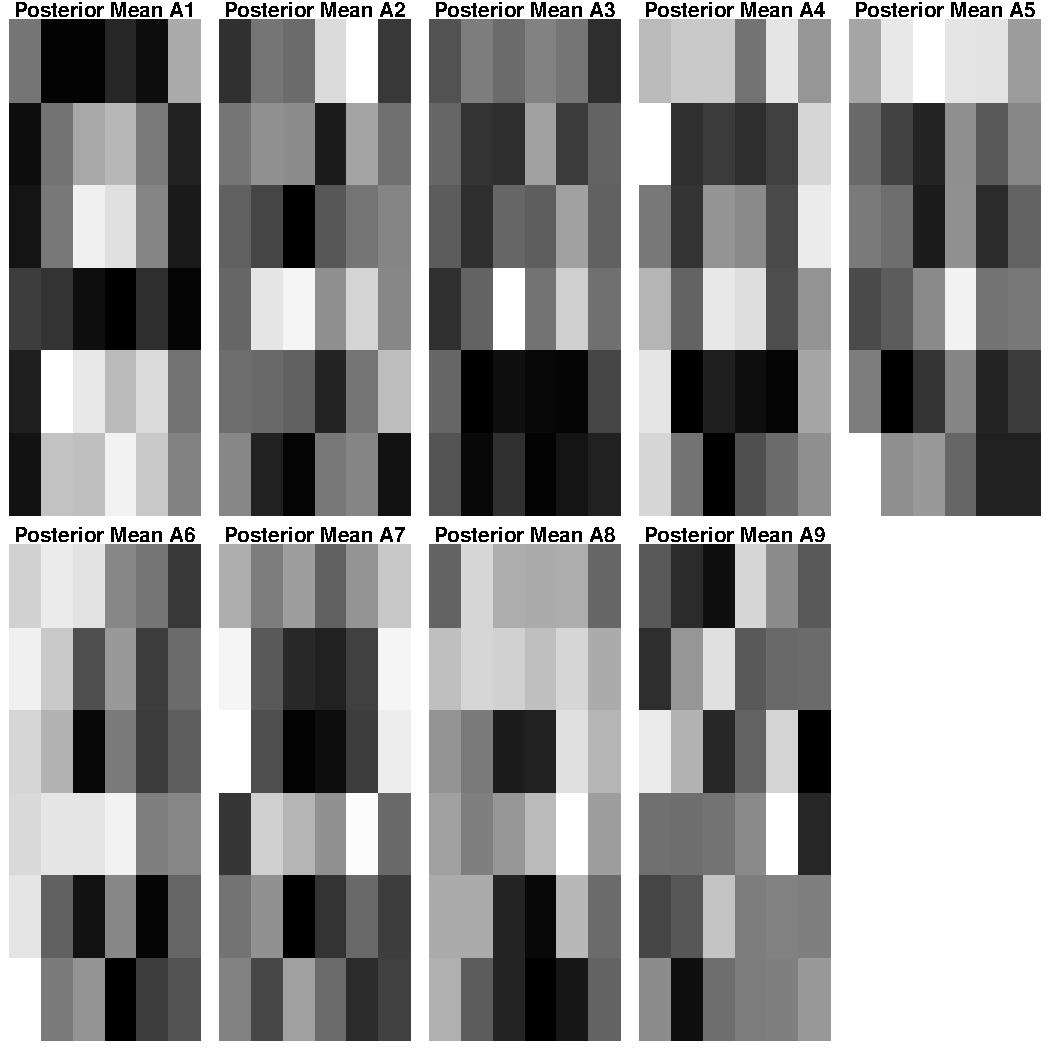
\includegraphics[height=1\textwidth]{images/postA66.pdf}
  \includegraphics{images/eSim.pdf}
  \caption{Expected value of the IBP, AIBP, and ddIBP, with $\alpha=2$, and 
           distance matrix D as shown in Table 4.1. }
\end{center}\end{figure}

\noindent
Figure 4.3 shows the expected values of the IBP, AIBP, and ddIBP, when the
first two rows are predetermined. In this case, the first two columns of the
first row were set to `1'; and the third and fourth columns of the second row
were set to `1'. It is clear that the distance information is respected in both
the ddIBP and the AIBP. It appears that in the AIBP, customers that are close
to one another tend to share the same dishes. Customer 3 is close to customer
1, and consequently takes dishes 1 and 2 more frequently than he would in the
IBP.  Customer 4 is far away from all other customers. Are more accurately, he
is equidistant from all other customers. So distance information does not have
an effect on him. He takes dishes with probabiltiy proportional to their
popularity, and not proportional to his proximity to customers that have taken
those dishes. Customer 5 tends to take dishes 3 and 4 because he is close to
customer 2, who has taken those dishes. In the ddIBP, customers that are far
apart tend to not share dishes. Instead of taking previously sampled dishes,
customer 4 samples more new dishes. 

\begin{figure}\begin{center}
  %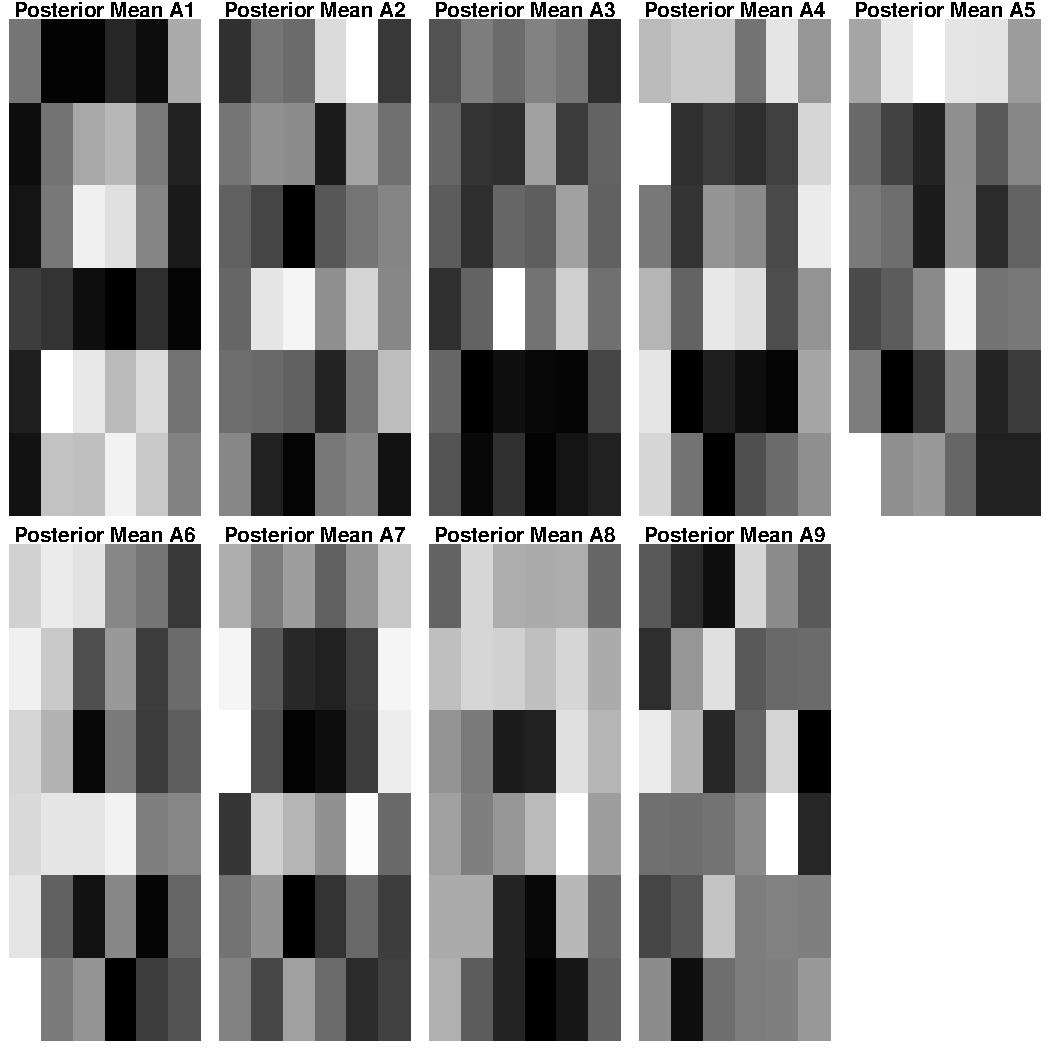
\includegraphics[height=1\textwidth]{images/postA66.pdf}
  \includegraphics{images/eSimFixed.pdf}
  \caption{Expected value of the IBP, AIBP, and ddIBP with $\alpha=2$, and
           distance matrix D as shown in Table 4.1, with the first two rows
           pre-set.}
\end{center}\end{figure}


\section{Comparisons between the AIBP \& ddIBP}
One obvious difference between the AIBP and ddIBP is that the pmf for any given
binary matrix can be evaluated for the AIBP, while the pmf cannot be explicitly
computed. For both the AIBP and ddIBP, expected row sums for a given parameter
$\alpha$ is $\alpha$, which is also the expected row sum for the IBP($\alpha$).
The expected number of non-zero columns in the AIBP is $\alpha H_N$, which is
also the expected number of non-zero columns in the IBP. This is because in the
AIBP, the process for each ``customer" drawing new dishes is the same as in the
IBP. This equality does not hold for the ddIBP. In general, expected column
sums are not equal to the IBP, for both the AIBP and ddIBP. However, the
expected matrix sums for both the AIBP and ddIBP are the same as that of the
IBP. The table below summarizes these findings. One implication of this result
is that the AIBP preserves the dimensions of the IBP, but redistributes
``dishes" to each customer based on proximity to other customers. The ddIBP
does not preserve the dimensions of the IBP in this manner. \\

\begin{center}
  \begin{tabular}{c|c|c}
    \hline
      Comparison & AIBP & ddIBP \\ \hline \hline
      Explicit pmf & Yes & No \\ \hline
      Expected non-zero columns equal to that of IBP & Yes & No \\ \hline
      Expected row sums equal to that of IBP & Yes & Yes \\ \hline
      Expected column sums equal to that of IBP & No & No \\ \hline
      Expected matrix sum equal to that of IBP & Yes & Yes \\ \hline
    \hline
  \end{tabular}
  \captionof{table} {Comparisons of the AIBP to the ddIBP showing how what 
                     properties of the IBP they presrve.}
\end{center}

